\documentclass[12pt]{article}
\usepackage{latexsym}
\usepackage{amssymb,amsmath}
\usepackage[pdftex]{graphicx}
\usepackage{color}
\usepackage{tikz}
\usepackage[margin=0.9in]{geometry}


\topmargin = 0.1in \textwidth=5.7in \textheight=8.6in

\oddsidemargin = 0.2in \evensidemargin = 0.2in


\begin{document}

\begin{center}
COMPUTER SCIENCE 20, SPRING 2014 \\
Homework Problems\\
Conditional Probability, Bayes Theorem, Expectations \\
Author: Tawheed Abdul-Raheem
\end{center}

\smallskip

\begin{enumerate}
\item Consider the strange dice from the last homework, which are 10-sided and have the property that the probability of rolling $n$ is \emph{proportional} to $n$. Imagine a situation in which you roll one of these dice, and then flip $m$ coins, where $m$ is the die roll. What is the probability of flipping at least 8 heads? Express your answer as a fraction; please do not compute a decimal. \\
  \textbf{Solution: } The probabilityof flipping 8 heads is the the probability of rolling 8 and getting 8 heads, rolling 9 and and getting 8 heads, rolling 9 and getting 9 heads, rolling 10 and getting either 10, 9 or 8 heads
  \[\text{Roll 8 $\cap$ 8 Heads } = \text{P(8 Heads $|$ Roll 8) $\cdot$ P(Roll 8)} \]
  \[\frac{\dbinom{8}{8}}{2^{8}} \cdot \frac{8}{55} = \frac{1}{2^{8}} \cdot \frac{8}{55} = \frac{1}{2^{5} \cdot 55} \]
  \[\text{Roll 9 $\cap$ 8 Heads } = \text{P(8 Heads $|$ Roll 9) $\cdot$ P(Roll 9)} \]
  \[\frac{\dbinom{9}{8}}{2^{8}} \cdot \frac{9}{55} = \frac{9}{2^{8}} \cdot \frac{9}{55} = \frac{81}{2^{8} \cdot 55} \]
  \[\text{Roll 9 $\cap$ 9 Heads } = \text{P(9 Heads $|$ Roll 9) $\cdot$ P(Roll 9)} \]
  \[\frac{\dbinom{9}{9}}{2^{8}} \cdot \frac{9}{55} = \frac{1}{2^{8}} \cdot \frac{9}{55} = \frac{9}{2^{8} \cdot 55} \]
  \[\text{Roll 10 $\cap$ 8 Heads } = \text{P(8 Heads $|$ Roll 10) $\cdot$ P(Roll 10)} \]
  \[\frac{\dbinom{10}{8}}{2^{8}} \cdot \frac{10}{55} = \frac{45}{2^{8}} \cdot \frac{10}{55} = \frac{450}{2^{8} \cdot 55} \]
  \[\text{Roll 10 $\cap$ 9 Heads } = \text{P(9 Heads $|$ Roll 10) $\cdot$ P(Roll 10)} \]
  \[\frac{\dbinom{10}{9}}{2^{8}} \cdot \frac{10}{55} = \frac{10}{2^{8}} \cdot \frac{10}{55} = \frac{100}{2^{8} \cdot 55} \]
  \[\text{Roll 10 $\cap$ 10 Heads } = \text{P(10 Heads $|$ Roll 10) $\cdot$ P(Roll 10)} \]
  \[\frac{\dbinom{10}{10}}{2^{8}} \cdot \frac{10}{55} = \frac{1}{2^{8}} \cdot \frac{10}{55} = \frac{10}{2^{8} \cdot 55} \]
  $\big[\text{Roll 8 $\cap$ 8 Heads } \big] + \big[\text{Roll 9 $\cap$ 8 Heads } \big] +\big[\text{Roll 9 $\cap$ 9 Heads } \big] +\big[\text{Roll 10 $\cap$ 8 Heads } \big] +\big[\text{Roll 10 $\cap$ 9 Heads } \big] +\big[\text{Roll 10 $\cap$ 10 Heads } \big]$

\begin{center}
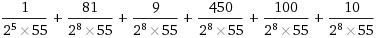
\includegraphics[scale=0.8]{quax.png}
\end{center}
\[\dfrac{329}{7040} \]

\item (Adopted from Meyer) Outside of their hum-drum duties as CS-20 Teaching Assistants, Nick is trying to learn to levitate using only intense concentration and Keenan is trying to become the world champion flaming torch juggler. Suppose that Nick’s probability of success is $1/6$, Keenan’s chance of success is $1/4$, and these two events are independent. \\\\
    T = Keenan (Torch juggling) \\
    L = Nick (Levitate)\\
\begin{enumerate}
\item If at least one of them succeeds, what is the probability that Nick learns to levitate? \\
  NB: \textbf{ATL} means at least \\
  \textbf{Solution }
  \[P(L | ATL 1) = \frac{P(ATL 1 | L) \cdot P(L)}{P(ATL 1)} \]
  Now we solve the fraction individually \\
  $P(ATL 1 | L) = 1$ \\
  $P(L) = \frac{1}{6}$ \\
  $P(ATL 1)$ has 3 possibilities \\
  $P(L \cap T) = P(L | T) \cdot P(T) = \frac{1}{6} \cdot \frac{1}{4} = \frac{1}{24} $ \\
  $P(L \cap \neg T) = P(L | \neg T) \cdot P(\neg T) = \frac{1}{6} \cdot \frac{3}{4} = \frac{3}{24}$ \\
  $P(\neg L \cap T) = P(\neg L | T) \cdot P(T) = \frac{5}{6} \cdot \frac{1}{4} = \frac{5}{24}$ \\
  \[\frac{{1} \cdot \frac{1}{6}}{\frac{9}{24}} = \frac{4}{29} \]
\item If at most one of them succeeds, what is the probability that Keenan becomes the world flaming torch juggler champion? \\
  NB: \textbf{ATM: } means at most \\
  $P(T | ATM 1) = \frac{P(ATM 1 \cap T)}{P(ATM 1)}$\\
Now we solve parts of the fraction inddividually \\
$P(ATM 1 \cap T) = P(\neg L \cap T)$ \\
$= P(\neg L | T) \cdot P(T)$ \\
$=P(\neg L) \cdot P(T)$ \\
$=\frac{5}{6} \cdot \frac{1}{4} = \frac{5}{24}$ \\
$P(ATM 1) $ has 3 possibilities \\
$P(T \cap \neg L) = \frac{1}{4} \cdot \frac{5}{6} = \frac{5}{24}$ \\
$P(L \cap \neg T) = \frac{1}{6} \cdot \frac{3}{4} = \frac{3}{24}$ \\
$P(\neg T \cap \neg L) = \frac{5}{6} \cdot \frac{3}{4} = \frac{15}{24}$\\
\[\frac{\frac{5}{24}}{\frac{23}{24}} = \frac{5}{23} \]
\item If exactly one of them succeeds, what is the probability that it is Nick? \\
  NB: \textbf{EX: } means exactly \\
  $P(Nick | EX 1) = \dfrac{P(EX 1 \cap Nick)}{P(EX 1)} $ \\
  Exactly 1 has two possibilities \\
  $P(L \cap \neg T) = \frac{1}{6} \cdot \frac{3}{4} = \frac{3}{24}$ \\
  $P(\neg L \cap T) = \frac{5}{26} \cdot \frac{1}{4} = \frac{5}{24}$ \\
  \[ \dfrac{P(EX 1 \cap L)}{P(EX 1)} = \dfrac{\frac{3}{24}}{\frac{8}{24}} = \dfrac{3}{8} \]
\end{enumerate}

\item A student in Monty Hall's probability course misses his exam and must take a makeup. Before the test, Prof. Hall invites him to choose one of five envelopes, two containing easy makeup exams, three containing hard ones, and the student takes an envelope.

``Before you start, you might enjoy looking at one of my hard makeup exams -- just full of nasty probability problems,'' says the professor. From among the four remaining envelopes, he selects one at random that he knows to contain a hard exam and opens it.

``Excuse me,'' says the student, ``but the envelope I picked looks a bit smudged. Could I swap it for one of the others?'' And he does.

What is the probability that the student has an easy exam after making the swap? \\
We can label $E$ as easy exams and $H$ as hard exams. There are 10 possible ways that the student can choose the first exams. After the first exams has been chosen, we can choose all the first hard ones from our 10 * 10 combination. We are left with 16 - Easy and 30 Hard leaving us with $\frac{16}{30}$
\[4 \cdot \dfrac{1}{3 \cdot 10} + 6 \cdot \dfrac{2}{3 \cdot 10} \]
\[\dfrac{4}{30} + \dfrac{12}{30} = \dfrac{16}{30} \]

\item (Adopted from Meyer) A 52-card deck is thoroughly shuffled and you are dealt a hand of 13 cards. 
  \begin{enumerate}
    \item If you have one ace, what is the probability that you have a second ace? \\
      $P(2A | 1A) = \dfrac{P(1A | 2A) \cdot P(2A)}{P(1A)}$ \\
      \[ \dfrac{1 * \bigg[  \dbinom{48}{11} \cdot \frac{\dbinom{4}{2}}{\dbinom{52}{13}} + \dbinom{48}{10} \cdot \frac{\dbinom{4}{3}}{\dbinom{52}{13}} + \dbinom{48}{9} \cdot \frac{\dbinom{4}{4}}{\dbinom{52}{13}} \bigg]}{\dbinom{48}{12} \cdot \frac{\dbinom{4}{1}}{\dbinom{52}{13}} + \dbinom{48}{11} \cdot \frac{\dbinom{4}{2}}{\dbinom{52}{13}} + \dbinom{48}{10} \cdot \frac{\dbinom{4}{3}}{\dbinom{52}{13}} + \dbinom{48}{9} \cdot \frac{\dbinom{4}{4}}{\dbinom{52}{13}}} = \dfrac{}{} \]

\begin{center}
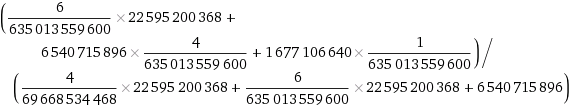
\includegraphics[scale=0.8]{q2.png}
\end{center}
\[ 3.934354251214668227689464737294999215548860642 × 10^{-11} \]
    \item If you have the ace of spades, what is the probability that you have a second ace? Remarkably, the answer is different from part (a). \\
      NB: \textbf{ATL: } means at least, \textbf{E: } means exactly. 
      \[\frac{P(A | ATL 2) \cdot P(ATL 2)}{P(A)} = \frac{P(A \cap E 2 A) + P(A \cap E 3 A) + P(A \cap E 4 A)}{P(A)} \]
      \[\dfrac{\bigg[\frac{1}{2} \cdot \dbinom{48}{11} \cdot \frac{\dbinom{4}{2}}{\dbinom{52}{13}} \bigg] + [\frac{3}{4} \cdot \dbinom{48}{10} \cdot \frac{\dbinom{4}{3}}{\dbinom{52}{13}} \bigg] + [\frac{2}{2} \cdot \dbinom{48}{9} \cdot \frac{\dbinom{4}{4}}{\dbinom{52}{13}} \bigg]}{\frac{1}{4}} = \dfrac{}{} \]
      \[  = 0.56115246098439375750300120048019207683073229291716680 \]
\end{enumerate}

\item \begin{enumerate}

\item Random variable $X$ can have the value -1, 1, 2, or $\frac{1}{2}$. Suppose that $P(X = 2) = P(X = \frac{1}{2}) = \frac{1}{3}$. Find values $a = P(X = 1)$ and $b = P(x = -1)$ such that $E(X) = 1$.
$ P(X = 2) = 1/3$\\
$P(X = 1/2) = 1/3$\\
$P(X = 1) = a$\\
$P(X = -1) = b$\\
$E(X) = P(X=2)*2 + P(X=1/2)*1/2 + P(X=1)*1 + P(X=-1)*(-1)$\\
$1 = 1/3*2 + 1/3*1/2 + a*1 + b*(-1)$\\
$1/3 + 1/3 + a + b = 1$\\
$a = 1 - 1/3 - 1/3 - b$\\
$a = 1/3-b$\\
$1 = 1/3*2 + 1/3*1/2 + (1/3-b)*1 + b*(-1)$\\
solve for b and that is the answer \\
$1 = 2/3 + 1/6 + (1/3-b) - b$\\
$b + b = 2/3 + 1/6 + 1/3 - 1$\\
$2b = 1/6 + 1 - 1$\\
$b = (1/6)/2 = 1/12$\\
a = $(a = 1/3 - b = 1/3 - 1/12 = 1/4)$\\
\item Random variable $Y$ can have only the value 2 or the value $\frac{1}{2}$, and for each of those values the probability is greater than zero. Show that $E(Y) \neq \frac{1}{E(\frac{1}{Y})}.$\\\\
Hint: Find a quadratic equation that must be satisfied by\\ the probability $a = P(Y = 2).$
  We prove by contradiction that the above equation is not true \\\\
  Y is 2 or $\frac{1}{2}$\\
  $P(2) > 0 \text{ and } P(1/2) > 0, \text{ where } P(Y = 2) > 0 \text{ and } P(Y = 1/2) > 0$ \\
  $E( Y) = 1/(E(1/Y))$ \\
  $E(Y ) = P(Y=2)*2 + P(Y=1/2)*1/2$ \\
  $E(1/Y) = P(1/Y = 2)*2 + P(1/Y = 1/2)*(1/2)$ \\
  $P(1/Y = 2) = P(Y = 1/2)$ \\
  $P(1/Y = 1/2) = P(Y = 2)$\\
  $E(1/Y) = P(Y=1/2)*2 + P(Y=2)*1/2$ \\
  $P(Y=2) = a$\\
  $P(Y=1/2) = 1-a$\\
  $E(Y ) = 1/(E(1/Y))$ \\
  $P(Y=2)*2 + P(Y=1/2)*1/2 = 1/(E(1/Y))$\\
  $ P(Y=2)*2 + P(Y=1/2)*1/2 = 1/( P(Y=1/2)*2 + P(Y=2)*1/2))$ \\
  $ [a *2 + (1 - a)*1/2] = [1/( 1-a)*2 + a*1/2)] $\\\\

From the above there is no way to get an $a$ that will make the equation equal.
The above equation was verified with WolframAlpha

\end{enumerate}

\end{enumerate}



\end{document} 
